\chapter{Mathematical Modelling}\label{ch:mathmodel}

\todo[color=04mathematicalModelling,inline]{break this chapter into static and dynamic modelling}
Most physical systems can be modelled statically or dynamically.
Depending on the application of the model,
and therefore on the end goal of the controller,
either option has some benefits and flaws.

Since our focus shifted during the project, we started out developing a static model,
describing the steady state response of the system.
Later on we decided to move towards a dynamic model, for easier PID-controller development.

Both modelling processes are described in this chapter,
with a small section in the end explaining the key differences.
\todo[color=04mathematicalModelling]{write a small conclusion at the end of this chapter}
\section{Static Modelling}\label{sec:statmod}

The static model explains the behaviour of the system at steady-state,
i.e. when the output is settled after a step input.
Static models are therefore also referred to as steady-state models.
Both expressions are used interchangeably throughout this report.

Typical static models for pump systems are pump curves and system curves.
%\todo[color=04mathematicalModelling,inline]{explain differences between pump curves and system curves}
%\todo[color=04mathematicalModelling,inline]{make sure sections and subsection makes sense}

\newpage
<<<<<<< Updated upstream

=======
We used the data gathered through experiments to develop a model that would fit all our data,
within a certain degree of error, and around an operating point. A model that could fit all the 
data within a small percentage error would be very hard to determine.

We decided to use grey-box modelling with polynomial fitting.
We consider our approach as grey-box rather than black-box,
because we chose the degrees of the polynomials based on known and tested physical relations.

A very similar modelling process was already successfully used by Pedersen and Yang 
\cite{YangMultiPump2008} on the same setup.
The choice of degree for the polynomials was determined by the affinity laws \cite{Volk2014}
and supported by very good fit to the data.

ML Curve Fitting Toolbox (\textit{cftool}) \cite{cftool}
was used in order to find the polynomial coefficients most accurately describing the system.
>>>>>>> Stashed changes
\subsubsection{Single Pump Model}
Equations \ref{eq:pumpHeadModel} and \ref{eq:pumpPowerModel} represents a model that 
determines the head and the power, given the flow. 
Although the formula does not directly relate to the pump speed, it indirectly 
relates to it, due to the fact that only one possible pump speed $\omega$ exists for a given flow,
provided everything else remains constant.
\todo[color=04mathematicalModelling]{quote zhenyu paper again}

\begin{equation}
	H = \bar{a_{0}} \cdot Q^2 + \bar{a_{1}} \cdot Q + \bar{a_{2}}
	\label{eq:pumpHeadModel}
\end{equation}
\begin{equation}
	P = \bar{b_{0}} \cdot Q^3 + \bar{b_{1}} \cdot Q^2 + \bar{b_{2}} \cdot Q + \bar{b_{3}}
	\label{eq:pumpPowerModel}
\end{equation}


The coefficients are determined by the pump characteristics and can be experimentally identified.
Taking variable speed into account, the equations \ref{eq:pumpHeadModel}  and \ref{eq:pumpPowerModel}
will depend on the motor speed. The pump Affinity Laws state:

\begin{align*}
	\left(\frac{\omega_1}{\omega_2}\right)^1 = \frac{Q_1}{Q_2} && 
	\left(\frac{\omega_1}{\omega_2}\right)^2 = \frac{H_1}{H_2} &&
	\left(\frac{\omega_1}{\omega_2}\right)^3 = \frac{P_1}{P_2}	
\end{align*}

Assuming the pump model parameters ($\bar{a_{0}}$, $\bar{a_{1}}$, $\bar{a_{2}}$ and $\bar{b_{0}}$,
$\bar{b_{1}}$, $\bar{b_{2}}$, $\bar{b_{3}}$) described in equation \ref{eq:pumpHeadModel} and 
\ref{eq:pumpPowerModel} are obtained at a certain speed $\bar{\omega_{0}}$, 
this results in the following equation describing the pump at any speed $\omega$.

\begin{equation}
	H(\omega) = a_0 \cdot \omega^2 + a_1 \cdot \omega \cdot Q(\omega) + a_2 \cdot Q(\omega)^2
	\label{eq:pumpHeadModel2}
\end{equation}
\begin{equation}
	P(\omega) = b_0 \cdot \omega^3 + b_1 \cdot \omega^2 \cdot Q(\omega) + b_2 \cdot \omega \cdot Q(\omega)^2 + b_3 \cdot Q(\omega)^3
	\label{eq:pumpPowerModel2}
\end{equation}

\newpage
The coefficients can be determined as follows:
\begin{align*}
	a_0 = \frac{\bar{a_0}}{\bar{\omega_0^2}} && a_1 = \frac{\bar{a_1}}{\bar{\omega_0}} && a_2 = \bar{a_2} \\
	b_0 = \frac{\bar{b_0}}{\bar{\omega_0^3}} && b_1 = \frac{\bar{b_1}}{\bar{\omega_0^2}} && b_2 = \frac{\bar{b_2}}{\omega_0} && b_3 = \bar{b_3}
\end{align*}

As observed in equations \ref{eq:pumpHeadModel2} and \ref{eq:pumpPowerModel2} the coefficients are
initially multiplied by the input speed. Afterwards they are divided by the
speed they were determined for, in order to take into account the variable speed.

Figure \ref{fig:flowVsPressure} shows data points connected together that represent 
a pump head curve. As observed in the figure, when the opening percentage of the control valve is at
10\% the pressure seems to reach negative values. We believe, this arises from the fact that we were not 
able to properly calibrate the pressure sensors. As an alternative, we have used the gain and offsets
provided to us by previous researchers that have experimented on the same setup. The gains and offsets
that we were able to determine for Flow and Power Consumption, respectively, were also consistent with
the values determined by us. This is the reason we decided to use the values provided to us.

\begin{figure}[h]
	\centering
	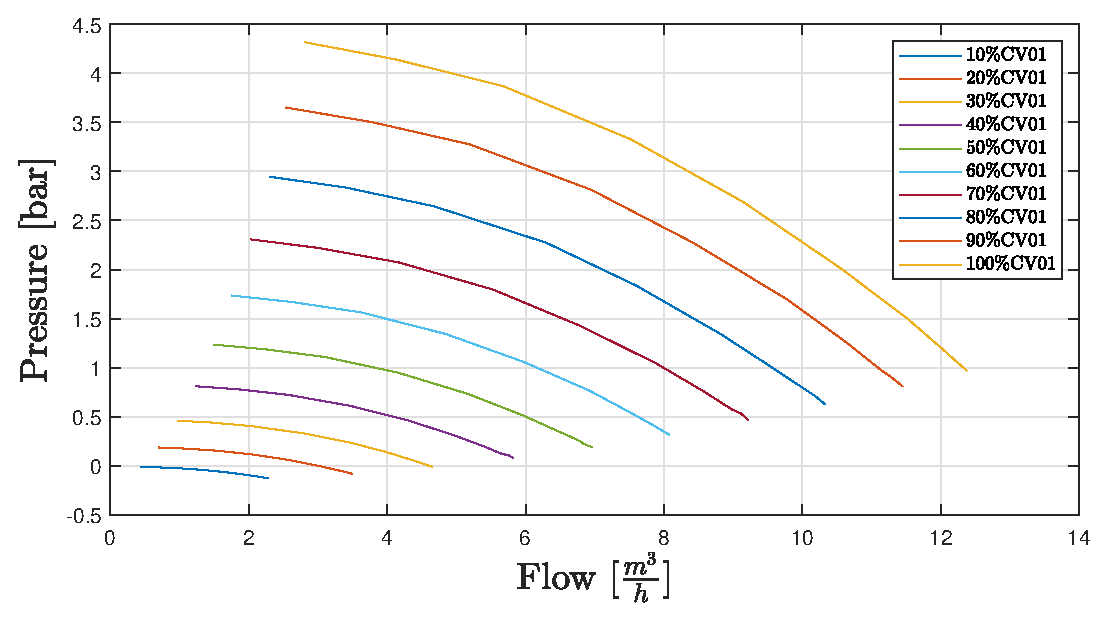
\includegraphics[width=1\textwidth]{figures/05mathematicalModelling/flowVsPressureRun34.eps}
	\caption{Data Points for Flow vs. Pressure}
	\label{fig:flowVsPressure}
\end{figure}

\newpage
Figure \ref{fig:flowVsPowerConsumption} shows data points connected together, representing a pump
power consumption curve.

\begin{figure}[ht]
	\centering
	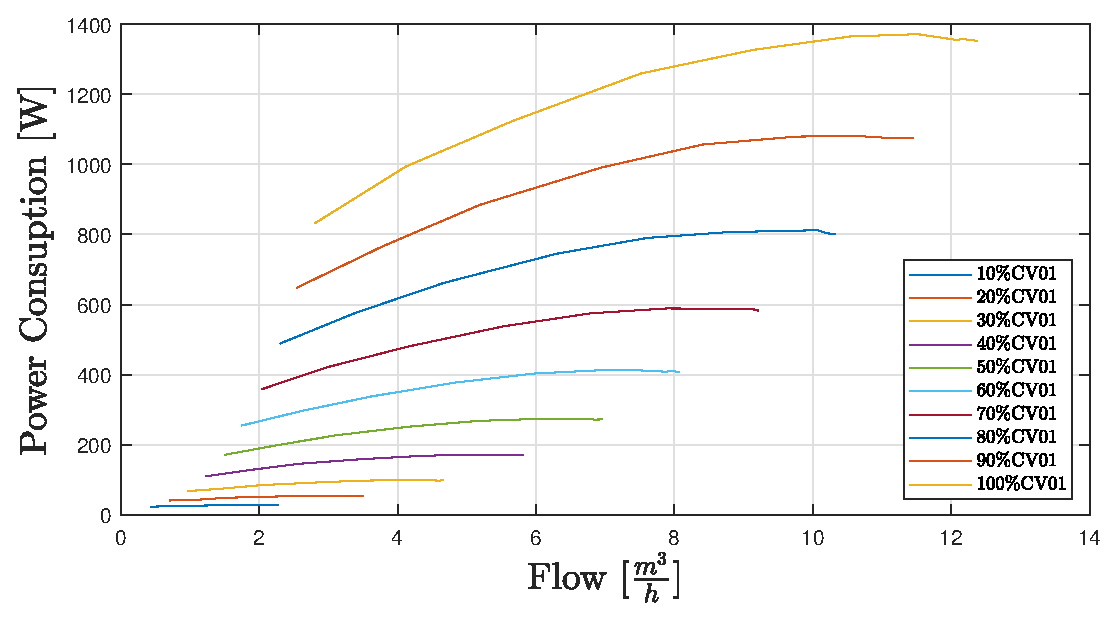
\includegraphics[width=1\textwidth]{figures/05mathematicalModelling/flowVsPowerRun34.eps}
	\caption{Data Points for Flow vs. Power Consumption}
	\label{fig:flowVsPowerConsumption}
\end{figure}

\textit{cftool} was used to determine coefficients  from each curve in  Figures \ref{fig:flowVsPressure}
and \ref{fig:flowVsPowerConsumption}.

%\newpage
%\subsubsection{Multiple Pumps Model at Same Speed}
%For a certain number of pumps P in parallel, with the requirement that they all run at the same speed
%$\omega$, the pump model is described by the following equations:

%\begin{equation}
%	\begin{aligned}
%	H_s(\omega) = a_0^s \cdot \omega^2 + a_1^s \cdot \omega \cdot Q_s(\omega) + a_2^s \cdot %Q_s(\omega)^2 \\
%	P_s(\omega) = b_0^s \cdot \omega^3 + b_1^s \cdot \omega^2 \cdot Q_s(\omega) + b_2^s \cdot \omega
%\cdot Q_s(\omega)^2 + b_3^s \cdot Q_s(\omega)^3
%	\end{aligned}
%\end{equation}

%The formulas are identical, however the coefficients differ. They can be determined as follows:
%\begin{align*}
%	a_0^s = a_0 && a_1^s = \frac{a_1}{P} && a_2^s = \frac{a_2}{P^2} \\
%	b_0^s = b_0 && b_1^s = \frac{b_1}{P} && b_2^s = \frac{b_2}{P^2} && b_3^s = \frac{b_3}{P^3}
%\end{align*}
%\todo[color=04mathematicalModelling]{very much from zhenyu's papers, should be able to understand and explain, otherwise, will take out and rewrite}

%\newpage
%The model has an adjusted coefficient of determination  $\bar{R^2}$ = 1. Such a high coefficient of determination, was achieved due to
%heavy filtering of the data gathered. In addition, no, or minor disturbances were present during the gathering of the data.
%\todo[color=04mathematicalModelling]{from supervisor meeting} 

%The model could be more expanded, reaching a higher order polynomial. However, we have decided the model represents the pump behavior 
%accurately enough. Further expansion would result in a higher degree polynomial but not much gain in terms of accuracy.

%Using the model shown in Equation \ref{eq:simulated_power} we were able to replicate our data with a small error percentage. The results
%are shown in the figures below.
%\todo[color=04mathematicalModelling]{not sure if we need this or not so i didn't put any photos}